\chapter{Implementation}
\label{chap:implementation}
The previous chapter demonstrated the architecture of the $\rho$-VEX processor and of the LLVM compiler. We have also shown that the LLVM compiler currently has support for a VLIW type processor. In this chapter we will show how the LLVM-based backend for the $\rho$-VEX processor has been implemented.

\section{Tablegen}
LLVM uses a domain-specific language (DSL) called \texttt{tablegen} to describe features of the backend such as instructions, registers, and pipeline information. 

\texttt{tablegen} uses a object-oriented approach to describe functionality. Information is described in classes and definitions that are called \emph{records}. Inheritance is supported so classes can derive information from superclasses. In addition, multiclasses can be used to instantiate multiple abstract records at once.

The \texttt{tablegen} tool aims to provide a flexible way to describe processor features. For example processor instructions could be described as follows:

A class is created that represents an abstract instruction. The class will describe information that is of direct importance to code generation such as opcode, register usage and immediate values but also information that is needed during the code generation such as liveness information, instruction pattern and scheduling information.

\begin{lstlisting}[language=tblgen]
class rvexInst<dag outs, dag ins, string asmstr, list<dag> pattern,
               InstrItinClass itin, Format f, CType type>: Instruction
{
}
\end{lstlisting}

The \texttt{rvexInst} class is used for all type of instructions that are supported by the $\rho$-VEX processor. Multiple instructions with common feature such as \texttt{add}, \texttt{sub}, and \texttt{and} can be described in subclasses that inherit from the \texttt{rvexInst} class. For example, the class \texttt{ArithLogicR} holds arithmetic instructions that use three register operands. The class describes common features such as the instruction string format and the instruction pattern that is used during instruction selection.

\begin{lstlisting}[language=tblgen]
class ArithLogicR<string instr_asm, SDNode OpNode,
                  InstrItinClass itin, RegisterClass RC, bit isComm = 0, CType type>:
  rvexInst <(outs RC:$ra), (ins RC:$rb, RC:$rc),
     !strconcat(instr_asm, "\t$ra = $rb, $rc"),
     [(set RC:$ra, (OpNode RC:$rb, RC:$rc))], itin, type> 
{
}
\end{lstlisting}

The following code shows how to define instructions that inherit from the \texttt{ArithLogicR} class. The instruction is defined as using the \texttt{ArithLogicR} class with certain parameters that match the instruction properties. These properties include instruction string, LLVM IR opcode, and other information that is needed during compilation.

\begin{lstlisting}[language=tblgen]
def ADD         : ArithLogicR<"add ", add, IIAlu, CPURegs, 1, TypeIIAlu>;
\end{lstlisting}

Figure \ref{fig:tblgen} displays an example of how individual instructions inherit from higher level classes. The final class is a \texttt{rvexInstr} that contains a description of all the available $\rho$-VEX instructions.

\begin{figure}[ht]
\centering
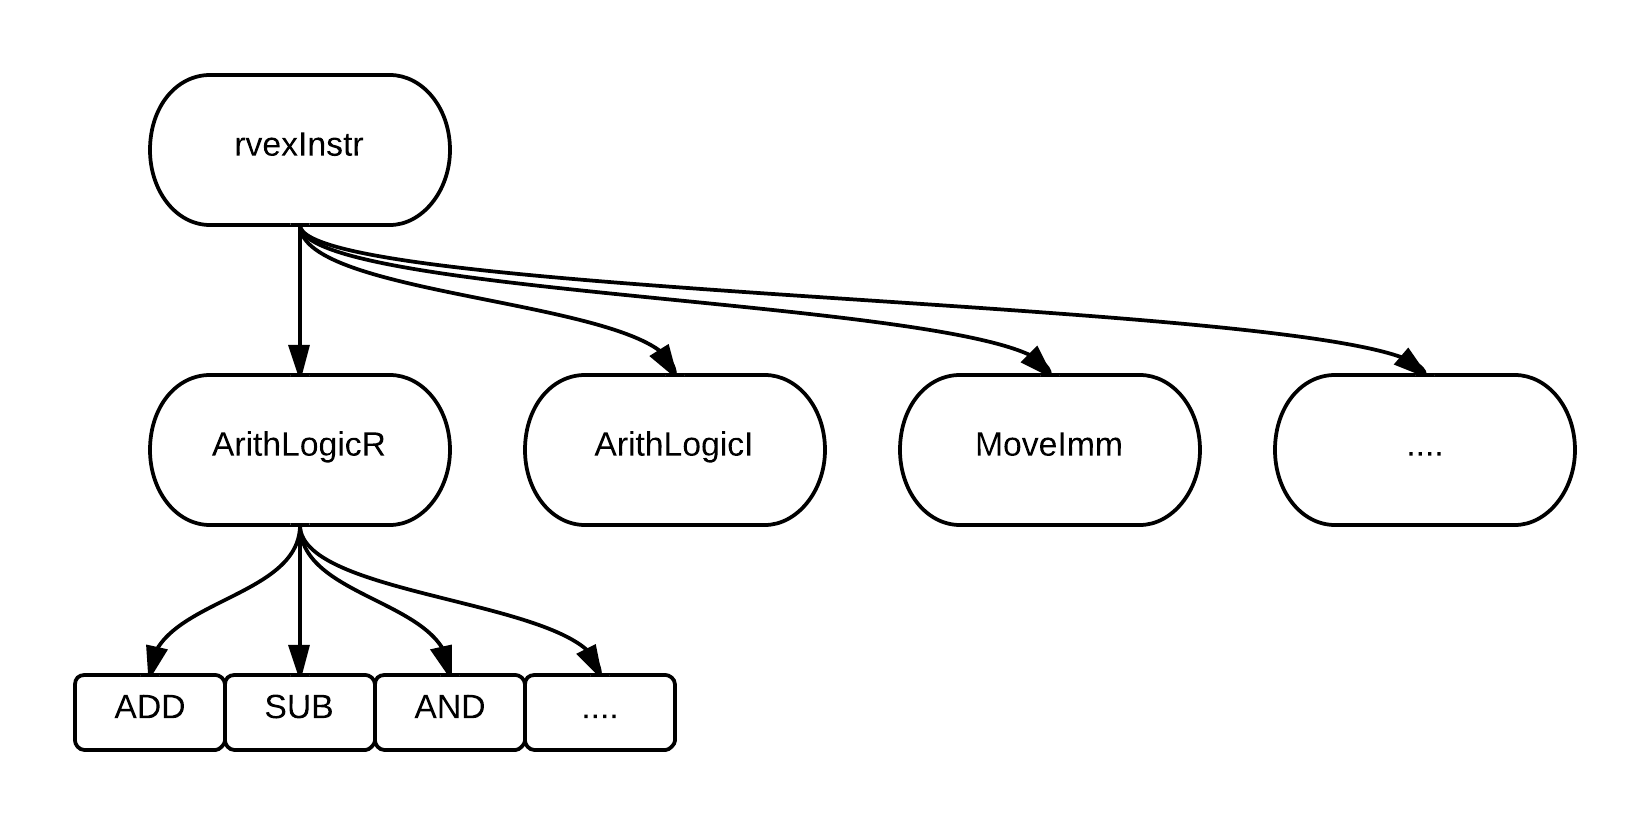
\includegraphics[width=0.8\textwidth]{3_implementation/img/instr.png}
\caption{\texttt{tblgen} instructions}
\label{fig:tblgen}
\end{figure}

\texttt{tablegen} provides for a very flexible way to describe backend functionality. The existing LLVM backends use \texttt{tablegen} in a variety of ways which best match the target processor. 

The \emph{tblgen} tool is used to transform the \texttt{tablegen} input files into C++. The resulting C++ files contain enums, structs and arrays that describe the properties. The instruction selection part is transformed into imperative code that is used by the backend for pattern matching. 

\subsection{Register definition}
LLVM uses a predefined class \texttt{register} to handle register classes. All $\rho$-VEX registers are derived from this empty class. The \texttt{rvexReg} class is used to define all type of $\rho$-VEX registers. 

\begin{lstlisting}[language=tblgen]
class rvexReg<string n> : Register<n> {
  field bits<7> Num;
  let Namespace = "rvex";
}
\end{lstlisting}

The \texttt{rvexReg} class is used to define the general purpose registers and the branch registers.
\begin{lstlisting}[language=tblgen]
class rvexGPRReg<bits<7> num, string n> : rvexReg<n> {
  let Num = num;
}

class rvexBRReg<bits<7> num, string n> : rvexReg<n> {
  let Num = num;
}
\end{lstlisting}

Each physical register is defined as an instance of one of these classes. For example, R5 is defined as follows. The register is associated with a register number, a register string, and a dwarf register number that is used for debugging.

\begin{lstlisting}[language=tblgen]
def R5 : rvexGPRReg< 5, "r0.5">, DwarfRegNum<[5]>;
\end{lstlisting}

The physical registers are divided in two register classes for the general purpose registers and for the branch registers. The register classes also define what type of value can be stored in the physical register.

\begin{lstlisting}[language=tblgen]
def CPURegs : RegisterClass<"rvex", [i32], 32, 
  (add
    (sequence "R%u", 0, 63),
    LR, PC
  )>;

def BRRegs   : RegisterClass<"rvex", [i32], 32, 
  (add 
    (sequence "B%u", 0, 7)
  )>;
\end{lstlisting}

The branch registers have been defined to also use 32 bit values even though in reality the branch register is only 1 bit wide. This has been done because LLVM had a lot of trouble identifying the correct instruction patterns for compare instructions. The $\rho$-VEX compare instruction can produce results in both the CPURegs and the BRegs as illustrated in the following example:

\begin{lstlisting}
<1 bit>BRRegs = Operation, <32 bit>CPURegs, <32 bit>CPURegs
<32 bit>CPURegs = Operation, <32 bit>CPURegs, <32 bit>CPURegs
\end{lstlisting}

The LLVM compiler is unaware that when the compare instruction is used to define a 32-bit result only the lowest bit will be set. The compiler tried to resolve this issue by inserting \texttt{truncate} and \texttt{zero\_extend} instructions even though this is not required. This has been solved by implementing the BRRegs as 32 bit wide so LLVM will not insert truncate and extend instructions when operating on these type of instructions.

\subsection{Pipeline definition}
\texttt{tablegen} can be used to describe the architecture of the processor in a generic way. LLVM will schedule an instruction to a processor functional unit during the scheduling pass. The following code describes the available functional units for a 4-issue a $\rho$-VEX processor.

\begin{lstlisting}[language=tblgen]
def P0 : FuncUnit;
def P1 : FuncUnit;
def P2 : FuncUnit;
def P3 : FuncUnit;
\end{lstlisting}

Each instruction is associated with an instruction itinerary. An instruction itinerary is used to group scheduling properties of instructions together. The $\rho$-VEX processor uses the following instruction itineraries.

\begin{lstlisting}[language=tblgen]
def IIAlu              : InstrItinClass;
def IILoadStore        : InstrItinClass;
def IIBranch           : InstrItinClass;
def IIMul              : InstrItinClass;
\end{lstlisting}

The functional units and instruction itineraries are used to describe the properties of the $\rho$-VEX pipeline. The scheduling properties are derived from a description of an instruction stage with certain properties and the associated instruction itinerary. These properties include the \emph{cycle count}, that describes the length of the instruction stage, and the functional units that can execute the instruction. The following itinerary describes a $\rho$-VEX pipeline with four functional units. Each functional unit is able to execute every instruction except for load / store instructions. Only \texttt{P0} is able to execute load / store instructions. These instructions take two cycles to complete.

\begin{lstlisting}[language=tblgen]
def rvexGenericItineraries : ProcessorItineraries<[P0, P1, P2, P3], [], [
  InstrItinData<IIAlu              , [InstrStage<1,  [P0, P1, P2, P3]>]>,
  InstrItinData<IILoadStore        , [InstrStage<2,  [P0]>]>,
  InstrItinData<IIBranch           , [InstrStage<1,  [P0, P1, P2, P3]>]>,
  InstrItinData<IIIMul             , [InstrStage<1,  [P0, P1, P2, P3]>]>,
]>;
\end{lstlisting}

The machine model class is used to encapsulate the processor itineraries and certain high-level properties such as issue width and latencies.

\begin{lstlisting}[language=tblgen]
def rvexModel : SchedMachineModel {
  let IssueWidth = 2;
  let Itineraries = rvexGenericItineraries;
}
\end{lstlisting}

\subsection{Other specifications}
\texttt{tablegen} is also used to describe other properties of the target processor. LLVM has stated as goal to move more parts of the backend description to the \texttt{tablegen} format because \texttt{tablegen} offers such a flexible implementation. At the moment \texttt{tablegen} is also used to implement:

\begin{itemize}
  \item Calling convention
  \item Subtarget features
\end{itemize}

\section{Code generation}
To understand how the compiler changes code from the LLVM IR representation to VEX assembly instruction it is necessary to understand how the code generation process works. The code generation process is divided into multiple steps, called passes, which are performed in order. 

\subsection{Instruction transformation}
The instruction selection phase is completed in the following steps
\begin{itemize}
  \item \textbf{Build initial DAG:} Transform the LLVM IR into a DAG that contains illegal types and instructions. The initial DAG is a one-to-one representation of the LLVM IR code.
  \item \textbf{Legalize instructions:} Illegal instructions are expanded and replaced with legal instructions.
  \item \textbf{Legalize types:} Transform the types used in the DAG to types that are supported by the target processor 
  \item \textbf{Instruction selection:} The legalized DAG still contains only LLVM IR instructions. The DAG is transformed to a DAG containing target-specific processor instructions.
\end{itemize}

\subsection{Instruction Lowering}
The \texttt{rvexISelLowering} class gives a high-level description of the operations that are supported by the target processor. The class can describe how the compiler should handle each LLVM IR instruction using four parameters: Legal, Expand, Promote or Custom. The default option is Legal, which implies that the LLVM IR instruction is natively supported by the target processor.

\subsubsection{Expanded instructions}
The Expand flag is used to indicate that the compiler should try to expand the instruction into simpler instructions. 
For example consider the LLVM IR \texttt{UMUL\_LOHI} instruction. This instruction multiplies two values of type \texttt{iN} and returns a result of type \texttt{i[2*N]}. Through expansion this instruction will be transformed into two mult instructions that calculate the low part and the high part separately.

\begin{lstlisting}[language=c] 
setOperationAction(ISD::UMUL_LOHI,  MVT::i32, Expand);
\end{lstlisting}

\subsubsection{Promote instruction}
Some instruction types are not natively supported and the type should be promoted to a larger type that is supported by the target processor. This feature is useful for supporting logical operations on Boolean functions. The following operation transforms an AND instruction that operates on a boolean value to a larger type.

\begin{lstlisting}[language=c] 
setOperationAction(ISD::AND,        MVT::i1, Promote);
\end{lstlisting}

\subsubsection{Custom expansion}
There are some instructions that cannot be expanded automatically by the compiler. To support these instructions the instruction expansion can be defined manually. For example consider the MULHS instruction that multiplies two numbers and returns the high part.

\begin{lstlisting}[language=c] 
setOperationAction(ISD::MULHS,      MVT::i32, Custom);
\end{lstlisting}

When a MULHS instruction is parsed the compiler will execute a function that describes the sequence of operations to lower this instruction. This sequence of instructions is implemented in the \texttt{LowerMULHS} function of the \texttt{rvexISelLowering} class. The \texttt{LowerMULHS} function is used to manually traverse the DAG and insert a sequence of instructions to support the operation.

For each instruction that requires custom lowering a \texttt{LowerXX} function has been defined.

\subsection{Instruction selection}
After instruction lowering the DAG contains LLVM IR operations and types that are all supported by the target processor but the DAG still contains only LLVM IR operations and no target-specific operations. The \texttt{rvexISelDAGToDag} class is used to match LLVM IR instructions to instructions of the target processor. The bulk of this class is generated automatically from the \texttt{tablegen} description but instructions can also be matched manually.

\subsection{New instructions}
The $\rho$-VEX processor supports some instructions that have no equivalent LLVM ISD operation. These instructions include \texttt{divs}, \texttt{addcg}, \texttt{min}, \texttt{max}, and others. Two stages are required to add support for these operations:

\begin{enumerate}
  \item \textbf{Extend ISD namespace:} The new instructions will be added to the ISD namespace. This means that the LLVM IR will be \emph{extended} with the new instructions.
  \item \textbf{Instruction lowering:} Describe when these instruction should be inserted in the LLVM IR. For example, lowering of the LLVM IR \texttt{div} instruction uses a custom lowering function to describe the algorithm that uses the $\rho$-VEX \texttt{divs} instruction.
  \item \textbf{Instruction matching:} New pattern matching rules need to be defined that map a custom instruction from the extended ISD namespace to the final target-specific $\rho$-VEX instructions.
\end{enumerate}

For this example we are going to consider the $\rho$-VEX \texttt{divs} instruction.

\subsubsection{Extend ISD namespace}
The ISD namespace can be extended with target-specific operations by defining the instruction type and the instruction name. Because the \texttt{divs} instruction uses five operands a custom instruction type will be used. The following code shows the definition for the custom instruction type. This type describes an instruction that produces two results and consumes three operands.

\begin{lstlisting}[language=tblgen]
def SDT_rvexDivs          : SDTypeProfile<2, 3
                                          [SDTCisSameAs<0, 2>,
                                          SDTCisSameAs<0, 3>,
                                          SDTCisInt<0>, SDTCisVT<0, i32>,
                                          SDTCisSameAs<1,4>,
                                          SDTCisInt<1>, SDTCisVT<1, i1>]>;
\end{lstlisting}

The next step involves defining the name of the custom instruction. The instruction is defined as a custom \texttt{SDNode} and uses the instruction type that has been defined earlier. This operation expands the LLVM ISD namespace with custom operations that are only available in the $\rho$-VEX backend.

\begin{lstlisting}[language=tblgen]
def rvexDivs              : SDNode<"rvexISD::Divs", SDT_rvexAddc>;
\end{lstlisting}

\subsubsection{Instruction lowering}
The \texttt{rvexISelLowering} class is extended with functions that produce the new ISD operation. For this example LLVM IR \texttt{div} instruction is custom lowered in the \texttt{LowerDIVS} function. In this function an algorithm is implemented that uses the new \texttt{divs} SDNode.

After instruction lowering a DAG will have been produced that contains only legal ISD operations and the new ISD operations that have been defined earlier.

\subsubsection{Instruction selection}
The following code describes the instruction class that is used by the \texttt{divs} instruction. This class describes the instruction string, register class properties and certain scheduling properties of this instruction. Note that the instruction pattern is empty because the current version of \texttt{tablegen} has no support for instructions that produce multiple results. A custom pattern matching function will need to be implemented in the \texttt{rvexISelDAGToDAG} class.

\begin{lstlisting}[language=tblgen]
class ArithLogicC<bits<8> op, string instr_asm, SDNode OpNode,
                  InstrItinClass itin, RegisterClass RC, RegisterClass BRRegs, bit isComm = 0, CType type>:
  FA<op, (outs RC:$ra, BRRegs:$co), (ins RC:$rb, RC:$rc, BRRegs:$ci),
     !strconcat(instr_asm, "\t$ra, $co = $rb, $rc, $ci"),
     [], itin, type> {        // Note empty instruction matching pattern
  let shamt = 0;
  let isCommutable = isComm;  // e.g. add rb rc =  add rc rb
  let isReMaterializable = 1;
}
\end{lstlisting}

The last step is to define the properties of the custom instruction.

\begin{lstlisting}[language=tblgen]
def rvexDIVS    : ArithLogicC<0x13, "divs ", rvexDivs, IIAlu, CPURegs, BRRegs, 1, TypeIIAlu>;
\end{lstlisting}

The \texttt{rvexISelDAGToDAG} class is used to define the custom instruction selection patterns. This class implements the pattern matching code that is generated from the \texttt{tablegen} description files. The class has a separate \texttt{select} function to match instructions that have no pattern matching rules defined.

The select function uses switch statements to select between custom \texttt{SDNodes}. The following function implements the pattern matching rule for the \texttt{divs} instruction that replaces the extended ISD \texttt{divs} instruction with the $\rho$-VEX instruction \texttt{rvexDIVS}. The \texttt{rvexDIVS} instruction has been defined earlier in the \texttt{tablegen} description files.

\begin{lstlisting}[language=C++]   
  case rvexISD::Divs: {
    SDValue LHS = Node->getOperand(0);
    SDValue RHS = Node->getOperand(1);
    SDValue Cin = Node->getOperand(2);
    return CurDAG->getMachineNode(rvex::rvexDIVS, dl, MVT::i32, MVT::i32,
                                  LHS, RHS, Cin);
    break;
  }
\end{lstlisting}

\subsubsection{Other cases}
Some $\rho$-VEX-specific instructions, such as the SHXADD instructions, are easier to support and do not need custom lowering. These instructions are also defined with empty pattern matching rules so the compiler will never insert them automatically. However the SHXADD instruction is easier to support because we can also match an instruction to a sequence of instructions. The following code describes a rule to replace the sequence \texttt{ADD (LHS\textless\textless1), RHS} with \texttt{SH1ADD LHS, RHS}.

\begin{lstlisting}[language=tblgen]
def : Pat<(add (shl CPURegs:$lhs, (i32 1)), CPURegs:$rhs),
          (SH1ADD CPURegs:$lhs, CPURegs:$rhs)>;
\end{lstlisting}

\subsection{Floating-point operations}
$\rho$-VEX processor does not natively support floating-point instructions. Instead software functions are used to execute FP operations. During instruction lowering FP operations are translated into library calls that will execute the instructions.

The LLVM compiler uses library functions that are compatible with the GCC Soft-FP library. The LLVM compiler-RT library is compatible with the GCC soft-FP library and is used for execution of FP instructions. Compiler-RT is a runtime library developed for LLVM that provides for these library functions.

\subsection{Scheduling}
During the scheduling pass the \texttt{SDNodes} are transformed into a sequential list form. Different schedulers are available for different processor types. For instance the register pressure scheduler will always try to keep the register pressure minimal which works better for x86 type processors. For the $\rho$-VEX processor a VLIW scheduler is used.

The list still does not contain valid assembly instructions. Virtual SSA based registers are still used and all the stack references do not reference true offsets.

\subsection{Register allocation}
During register allocation the virtual registers are mapped to available physical registers of the target processor. The register allocator considers the calling convention, reserved registers and special hardware registers during allocation. In addition the register allocator also inserts spill code when a register mapping is not available.

Liveness analysis is used to determine which virtual registers are used at a certain time. The liveness of virtual registers can be determined easily through the SSA based form of the input list. Multiple register allocation algorithms are available. All algorithms operate on the liveness information.

\subsection{Hazard recognizer}
The $\rho$-VEX processor has no way to recognize hazards or halt execution of code for a cycle. Because of this the correct scheduling of instructions is important for correct execution. Consider the following sequence of code:

\begin{lstlisting}[language=rvex]
  ldw $r0.2 = 0[$r0.2]  # Load from main memory
;;
  add $r0.2 = $r0.2, 2  # Add 2 to register
;;
\end{lstlisting}

After execution the register r0.2 will contain an undefined value because the load instruction has not completed execution. The compiler needs to insert an instruction or nop between the load and add instruction for correct execution. The correct instruction sequence should be the following:

\begin{lstlisting}[language=rvex]
  ldw $r0.2 = 0[$r0.2]  ## Load from main memory
;;
                        ## Empty instruction
;;
  add $r0.2 = $r0.2, 2  ## Add 2 to register
;;
\end{lstlisting}

The \texttt{ScheduleHazardRecognizer} is only able to resolve structural hazards, not data hazards. In Chapter \ref{chap:optimization} we will describe how the hazard recognizer has been combined with a new scheduling algorithm to resolve both data and structural hazards.

\subsection{Prologue and epilogue insertion}
After the register allocation pass the prologue en epilogue functions can be inserted. The prologue and epilogue pass is used to calculate the correct stack offset for each variable. Code is inserted that reserves room on the stack and saves / loads variables from the stackframe.

\subsection{VLIW Packetizer}
The packetizer pass is an optional pass that is used for VLIW targets. The packetizer receives a list of sequential machine instructions that need to be bundled for VLIW processors. 

The \texttt{tablegen} pipeline definition is used to build a DFA that represents the resource usage of the processor. The DFA can be used to determine to which functional unit an instruction can be mapped and if enough functional units are available.

The DFA representation is powerful enough to consider different properties of functional units. For example consider a 4-issue width VLIW processor but with only one unit supporting load / store operations. The DFA can model this pipeline and guarantee only one load / store instruction will be executed per clock cycle.

The VLIW packetizer also checks if certain instructions are legal to bundle together. The packetizer can be customized to check for hazards such as data dependency hazards, anti dependencies and output dependencies. Custom hazards can also be inserted to make sure that control flow instructions are always in a single bundle.

\section{New LLVM features}
This section describes features that have been added to the LLVM compiler. Currently, the $\rho$-VEX backend is the only backend that supports these kind of features.

\subsection{Generic binary support}
% FIXME uitleggen hoe instructies worden geserialized

By disallowing RAW hazards in instruction bundles, binaries can be generated that can execute on any $\rho$-VEX processor irrespective of issue width. For example consider the following instruction packet. The RAW hazard will occur on the r0.8 register.

\begin{lstlisting}[language=rvex]
  add $r0.10  = $r0.10, $r0.11
  add $r0.12  = $r0.12, $r0.13
  add $r0.14  = $r0.14, $r0.8
  add $r0.8   = $r0.8, $r0.9
;; 
\end{lstlisting}

Execution of this code on a 4-issue width processor will be fine but if this instruction is executed on a 2-issue width processor a problem will arise. The contents of register r0.8 will be changed during execution of the first bundle and execution of the second bundle will produce an invalid result.

This bundle should be split into two instructions during compilation. This can be achieved by checking for RAW hazards inside a bundle during the VLIW packetizer pass. The VLIW packetizer will detect these hazards and split the instructions into different bundles so correct execution is guaranteed.

\subsection{Compiler parameterization}
The HP VEX compiler supports a machine description file that describes properties of the processor. Using this machine description certain parameters, such as issue width, multiply units, load / store units, and branch units can be customized. 

Currently the LLVM compiler supports parameterization through subtarget support. Backend features can be enabled and disabled with command line parameters. The ARM backend uses this approach to select between different ARMv7 architectures, floating point support and div/mul support. This approach would not be useful for the $\rho$-VEX processor because of the amount of features that can be customized. Each customizable feature would need a new subtarget. For example, when four features can be customized (W, X, Y and Z), then $W*X*Y*Z$ subtargets would be needed. Clearly, this approach is not usable for the $\rho$-VEX processor where multiple parameters can be customized with a wide range of possibilities.

A different approach is used that changes the target description during runtime of the compiler. The target processor features are described in the \texttt{rvexMCTargetDesc} class. During runtime a machine description file will be read parsed and information from this machine description will be used to update the \texttt{rvexMCTargetDesc} class. 

The following properties can be customized through the machine description file:

\begin{itemize}
  \item \textbf{Generic binary:} disable RAW hazard check in VLIW packetizer
  \item \textbf{Width:} issue width of the processor
  \item \textbf{Stages:} describes all the available functional units an the amount of cycles an instruction fills a functional unit.
  \item \textbf{Instruction itinerary:} maps an instruction itinerary to a function unit. Also describes at what cycle the output contains a legal value.
\end{itemize}

The parameters are also used to generate the DFA that will track the resource usage. During the translation of the \texttt{tablegen} file an algorithm is used to generate a DFA from the available functional units. This algorithm has been implemented in the \texttt{rvexMCTargetDesc} class.

The location of the machine description file is passed to the \texttt{rvexMCTargetDesc} through command line parameters. Custom command-line parameters can be implemented in LLVM using \texttt{cl::opt} templates.

Some parameters such as the toggling of generic binary support is not handled through the \texttt{rvexMCTargetDesc} file. These parameters are used to set global state flags that can be read at anypoint in the compilation process. The \texttt{Is\_Generic\_flag} is used during the \texttt{rvexVLIWPacketizer} pass and during the liveliness calculation pass.

The following code demonstrates the configuration file for a 4-issue width  $\rho$-VEX processor with support for generic binaries. The \texttt{Stages} parameter uses three values. The first value describes the amount of clock cycles a instruction occupies a functional unit the second parameter is a bitmask for which functional unit can handle this instruction. The third parameter is currently not used.

The \texttt{InstrItinerary} parameter describes which type of instruction maps to which \texttt{Stage}. The first value describes which Stage an instruction is going to use, the second parameter describes when the result of the operation is available.

\begin{lstlisting}[language=config]
Generic         = 1;
Width           = 4; 
Stages          = {1, 15, 1}, {1, 1, 1}, {2, 2, 1};
InstrItinerary  = {1, 2}, {1, 2}, {3, 5}, {2, 3}, {1, 2}, {1, 2};
\end{lstlisting}

The compiler parameterization feature can be easily ported to other LLVM backends. The only part that has changed is the \texttt{rvexMCTargetDesc} class. 

\section{Conclusion}
In this section, we have shown how the $\rho$-VEX backend for the LLVM compiler has been implemented. Using the \texttt{tablegen} description we have described all the instructions that are supported by the $\rho$-VEX processor. We have also shown how LLVM IR code is transformed into a DAG that represents the original program. Through lowering functions this DAG is transformed into a DAG that contains only operations that are supported by the target processor. With instruction selection the DAG is transformed into a new DAG that contains target specific operations.

The finished DAG is transformed into a sequential list of instructions. This instruction list is used for the remaining passes. The remaining passes are used to map virtual registers to physical registers, emit prologue and epilogue functions and to perform VLIW packetization.

Support for floating-point operations has been added by porting the LLVM floating point library to the $\rho$-VEX processor.

Certain features that are required for the $\rho$-VEX processor were not available in the LLVM compiler. Features such as a machine description file are new to LLVM and we have shown what changes have been made to the LLVM compiler to support machine description files. In addition, we have shown how the backend has been updated to provide support for the $\rho$-VEX generic binary format.


\acresetall

